\documentclass[12pt]{article}

\usepackage[a4paper,margin=2.5cm]{geometry}
\usepackage{amsmath, amssymb, amsthm}
\usepackage{bm}
\usepackage{hyperref}
\usepackage{graphicx}
\usepackage{caption}
\usepackage{listings}
\usepackage{xcolor}
\usepackage{float}
\usepackage{placeins}
\graphicspath{{figures/}}

\lstdefinestyle{code}{
  basicstyle=\ttfamily\small,
  numbers=left,
  numberstyle=\tiny,
  numbersep=8pt,
  keywordstyle=\color{blue},
  commentstyle=\color{teal!70!black},
  stringstyle=\color{orange!70!black},
  showstringspaces=false,
  breaklines=true,
  frame=single,
  framerule=0.3pt,
  rulecolor=\color{black!15}
}
\lstset{style=code}

\title{Q-learning Tutorial}
\author{}
\date{\today}

\begin{document}
\maketitle

\section{Introduction}
Q-learning is an off-policy, model-free reinforcement learning algorithm that learns the optimal action-value function by interacting with an environment. By iteratively updating state-action values with bootstrapped targets, Q-learning converges to the optimal policy under mild assumptions even when actions are selected using exploratory behaviour such as \(\varepsilon\)-greedy strategies.

\section{Theory and Formulas}
\subsection{Action-Value Function}
For a Markov Decision Process (MDP) with states \(s \in \mathcal{S}\), actions \(a \in \mathcal{A}\), transition probability \(P\), and reward \(R\), the optimal action-value function satisfies the Bellman optimality equation
\begin{equation}
Q^*(s,a) = \mathbb{E} \big[ r_{t+1} + \gamma \max_{a'} Q^*(s_{t+1}, a') \mid s_t = s, a_t = a \big],
\end{equation}
where \(\gamma \in [0,1)\) is the discount factor.

\subsection{Update Rule}
Q-learning maintains an estimate \(Q_t\) that is updated after observing transition \((s_t, a_t, r_{t+1}, s_{t+1})\):
\begin{equation}
Q_{t+1}(s_t, a_t) \leftarrow Q_t(s_t, a_t) + \alpha_t \Big[ r_{t+1} + \gamma \max_{a'} Q_t(s_{t+1}, a') - Q_t(s_t, a_t) \Big],
\end{equation}
with learning rate \(\alpha_t\). Actions during data collection can follow an \(\varepsilon\)-greedy policy \(\pi(a|s)\) that selects the greedy action with probability \(1-\varepsilon\) and explores otherwise.

\subsection{Convergence Considerations}
If learning rates satisfy \(\sum_t \alpha_t = \infty\) and \(\sum_t \alpha_t^2 < \infty\), all state-action pairs are visited infinitely often, and rewards are bounded, Q-learning converges to \(Q^*\) with probability 1. In practice, constant learning rates and decaying exploration are used. Function approximation and large state spaces require variants such as Deep Q-Networks (DQN) with replay buffers and target networks.

\section{Applications and Tips}
\begin{itemize}
  \item \textbf{Game playing}: learn control policies in discrete environments (grid worlds, Atari) without explicit models.
  \item \textbf{Robotics and control}: discretized action spaces for navigation and low-level control.
  \item \textbf{Operations research}: optimize inventory management or queueing decisions via simulation.
  \item \textbf{Best practices}: normalize rewards, anneal exploration, monitor learning curves, and clip updates or rewards to stabilize training.
\end{itemize}

\section{Python Practice}
The script \texttt{gen\_q\_learning\_figures.py} simulates a 2D grid-world with terminal rewards, applies tabular Q-learning, and records episode returns and greedy state values for visualization.
\begin{lstlisting}[language=Python,caption={Excerpt from gen_q_learning_figures.py}]
for episode in range(num_episodes):
    state = env.reset()
    done = False
    G = 0.0
    while not done:
        action = epsilon_greedy(Q[state], epsilon)
        next_state, reward, done = env.step(action)
        best_next = np.max(Q[next_state])
        Q[state, action] += alpha * (reward + gamma * best_next - Q[state, action])
        state = next_state
        G += reward
    returns.append(G)
\end{lstlisting}

\section{Result}
\begin{figure}[H]
  \centering
  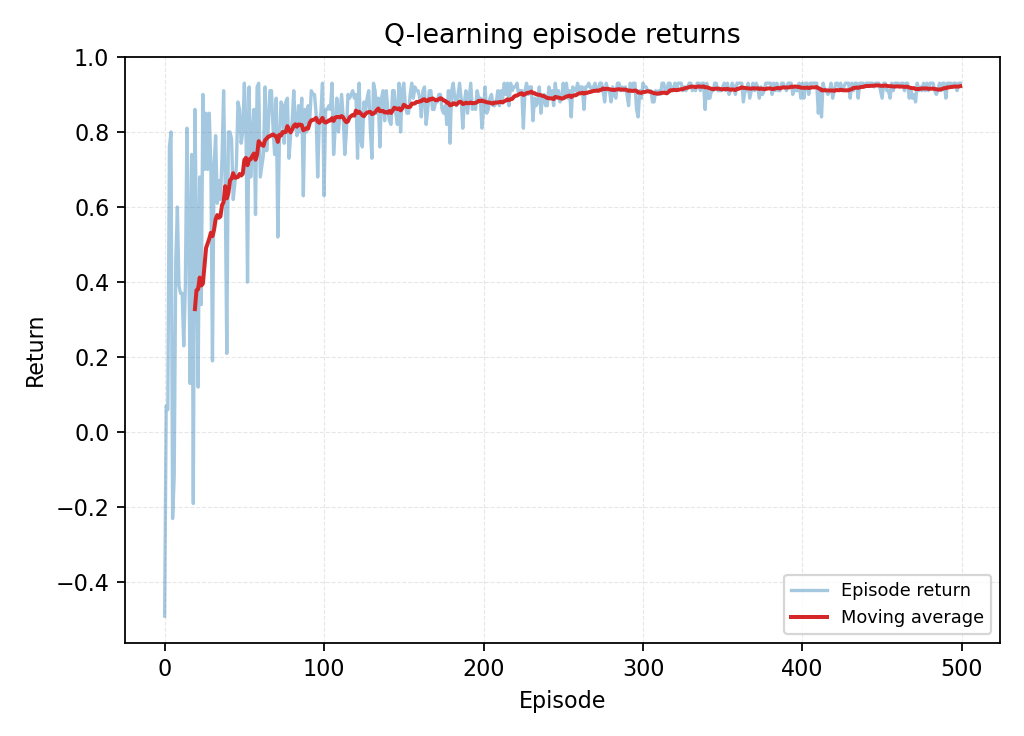
\includegraphics[width=0.8\linewidth]{q_learning_returns.png}
  \caption{Q-learning episode returns moving toward the optimal value}
  \label{fig:q_learning_returns}
\end{figure}

\begin{figure}[H]
  \centering
  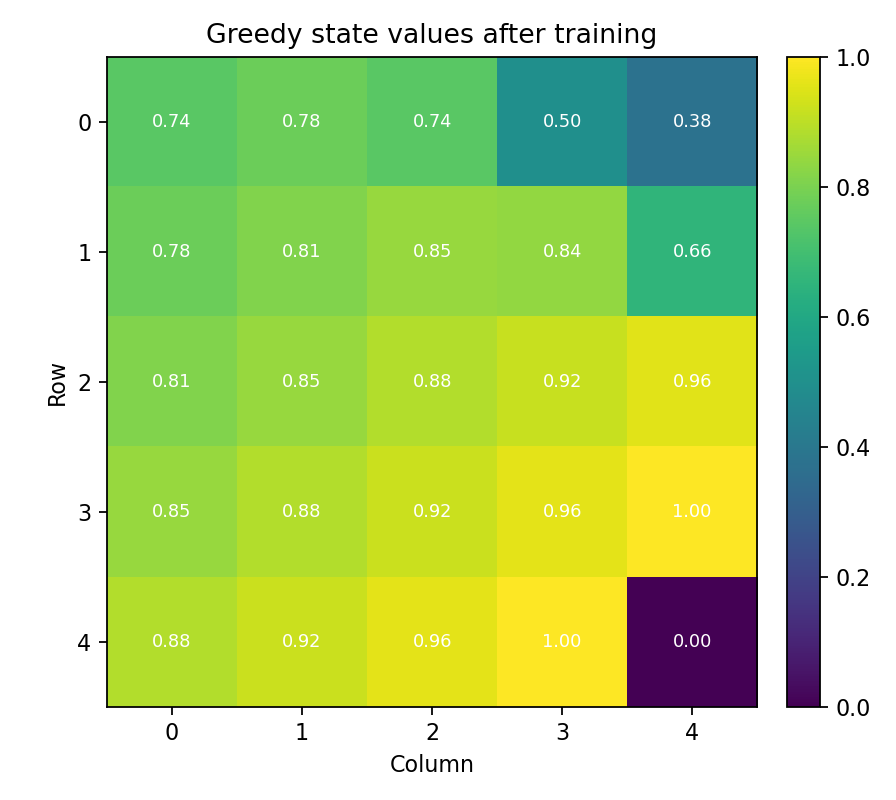
\includegraphics[width=0.82\linewidth]{q_learning_state_values.png}
  \caption{Heatmap of greedy state values after training, highlighting shortest-path structure}
  \label{fig:q_learning_state_values}
\end{figure}

\FloatBarrier
\section{Summary}
Q-learning estimates optimal action values via temporal-difference updates using max bootstrapping. Careful tuning of learning rate, exploration schedule, and reward scaling yields stable convergence. The grid-world example illustrates how episode returns improve over time and how learned state values encode optimal trajectories.

\end{document}